\subsection{Przegląd literatury}
\subsubsection{Wstęp}
Rozważania na temat inteligentnych systemów w kontekście niniejszej pracy należy rozpocząć od artykułu opublikowanego przez IBM w 2003 roku \cite{kephart2003}. Wskazuje on, iż ówczesne systemy informatyczne stawały się coraz bardziej złożone, co prowadziło do kryzysu zarządzania. Ręczna administracja przestawała być skalowalna, ponieważ systemy wymagały coraz większej liczby specjalistów do ich instalacji, konfiguracji oraz optymalizacji. IBM wskazywał, że jedynym rozwiązaniem tego problemu jest autonomiczne przetwarzanie (ang. \textit{Autonomic Computing}). Koncepcja ta nawiązuje do autonomicznego układu nerwowego człowieka, który zarządza pracą serca i regulacją temperatury ciała, odciążając świadomą część mózgu.

W kontekście systemów informatycznych oznaczałoby to zwolnienie człowieka z konieczności ręcznej konfiguracji, optymalizacji, naprawy oraz ochrony systemów, ponieważ miałyby one zdolność do samodzielnej adaptacji zgodnie z modelem (ang. \textit{Self-Configuration, Self-Optimization, Self-Healing, Self-Protection}). Jest to kluczowe pojęcie, które stanowi fundament wielu późniejszych badań nad autonomicznymi systemami. Architektura takich systemów została przedstawiona na rysunku \ref{fig:24-ibm}.

\begin{figure}[!htbp]
    \centering 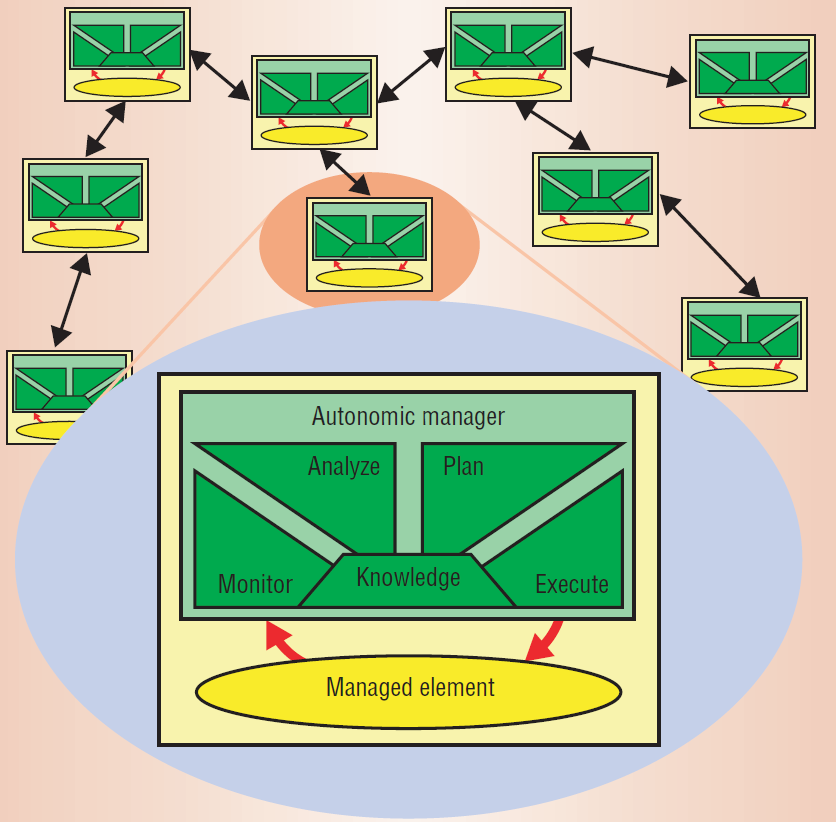
\includegraphics[width=1.0\linewidth]{24-ibm.png}
    \caption{Architektura autonomicznych systemów IBM. Źródło \cite{kephart2003}.}\label{fig:24-ibm}
\end{figure}

Podstawową jednostką systemu autonomicznego jest element autonomiczny (ang. \textit{Autonomic Element}). Składa się on z zarządzanego komponentu (np. serwera, bazy danych, aplikacji czy urządzenia sieciowego) oraz autonomicznego menadżera (ang. \textit{Autonomic Manager}), który steruje jego działaniem. Menedżer autonomiczny działa w cyklu MAPE-K (Monitor, Analyze, Plan, Execute, Knowledge). Faza "Monitor" zbiera dane o zarządzanym obiekcie, które następnie są analizowane i oceniane pod względem potencjalnych problemów w fazie "Analyze". "Plan" odpowiada za opracowanie działań naprawczych lub optymalizacyjnych, które są przekazywane do "Execute" w celu wdrożenia w systemie zarządzanym. "Knowledge" nie jest odrębną fazą, lecz repozytorium wiedzy, do której każdy z elementów cyklu ma dostęp. Tu gromadzona jest \hyperlink{def:wiedza}{\textit{wiedza}}. Elementy autonomiczne mogą ze sobą współpracować i wymieniać się wiedzą. Inteligencja społeczna (ang. \textit{social intelligence}) całego rozproszonego systemu zwiększa się wraz z liczbą interakcji pomiędzy elementami, podobnie jak w kolonii mrówek. Nowe elementy systemu mogą pozyskiwać wiedzę od pozostałych jednostek. Koncepcja ta wykazuje pewne podobieństwo do teorii przedstawionych przez Minsky'ego \cite{minsky1986}.

Następnie \cite{doyle2014} opisuje ewolucję architektury sieci telekomunikacyjnych w kierunku większej automatyzacji wymieniając czynniki umożliwiające (ang. \textit{enablers}) taki kierunek jako technologie: SDN (ang. \textit{Software Defined Networks}) oraz NFV (ang. \textit{Network Function Virtualization}).

Należy w tym miejscu rozróżnić pojęcia Automatyzacji i Autonomiczności. Pierwsze odnosi się do predefiniowanego i zaprogramowanego procesu, podczas gdy drugie do aspektów związanych z samozarządzaniem. Zazwyczaj proces automatyczny nie jest w stanie zaadaptować się do zmian środowiska bez interwencji człowieka, w przeciwieństwie do procesu autonomicznego \cite{ngmn2022}. Czynnikiem technologicznym (ang. \text{enabler}) pozwalającym na przejście z automatyzacji na autonomiczność jest sztuczna inteligencja. \cite{benzaid2020} dokonuje przeglądu kierunków rozwoju badań na temat bezobsługowych systemów zarządzania siecią i usługami (ang. \textit{Zero-touch network and Service Management}), gdzie sztuczna inteligencja odgrywa kluczową rolę. Artykuł wymienia projekty organizacji standaryzujących w tym obszarze:
\begin{itemize}
    \item \textbf{ETSI GS ZSM} - specyfikuje referencyjną architekturę zarządzania siecią i usługami end-to-end. Framework ZSM jest postrzegany jako system zarządzania nowej generacji, który ma na celu pełną autonomiczność wszystkich procesów - od planowania, projektowania, dostarczania i wdrażanie, po udostępnianie, monitorowanie i optymalizację. Docelowo, w idealnym przypadku, powinien on działać w 100\% samodzielnie bez ingerencji człowieka. 
    \item \textbf{TM Forum} - specyfikuje referencyjną architekturę CLADRA (Closed Loop Anomaly Detection and Resolution Automation) opartej na sztucznej inteligencji, która umożliwia dostawcom usług komunikacyjnych (CSP - ang. \textit{Communication Service Providers} na szybkie wykrywanie i rozwiązywanie problemów sieciowych.
    \item \textbf{ETSI GR ENI} - specyfikuje referencyjną architekturę kognitywnych systemów zarządzania siecią używając zamkniętych pętli sterowania oraz świadomych kontekstu polityk. O ile ETSI GS ZSM skupia się na technikach automatyzacji zarządzania oraz udostępniania usług end-to-end, to ENI koncentruje się na technikach AI, zarządzaniu poprzez polityki oraz zamkniętych pętlach sterowania.
\end{itemize}

Powyższe architektury zostaną dokładniej opisane w następnych podrozdziałach. Istotne na tym etapie jest to, ze każda z tych architektur opiera swoje działanie o zamknięte pętle sterowania, co przewidziano w \cite{fallon2019}. Artykuł wskazuje, iż badania nad zamkniętymi pętlami sterowania to dyscyplina o długiej historii, sięgająca aż epoki pary \footnote{\url{https://en.wikipedia.org/wiki/Age_of_Steam}} (Rysunek \ref{fig:24-his}). Z powodzeniem znajdują zastosowanie w systemach morskich, lotniczych, motoryzacyjnych, przemysłowych, ale też mikroprocesorach, systemach wbudowanych czy sterownikach urządzeń. Mimo że tego typu systemy są często złożone, cechują się determinizmem i dobrze określonymi granicami, co sprawia, że nadają się do zastosowania teorii sterowania\footnote{\url{https://en.wikipedia.org/wiki/Control_theory}}. Systemy telekomunikacyjne natomiast są słabo określonymi, stochastycznymi systemami, co sprawia, że zastosowanie teorii sterowania do ich zarządzania jest wyjątkowo trudne. To powoduje znaczne opóźnienie w adaptacji tych rozwiązań w branży telekomunikacyjnej. Od czasu pojawienia się koncepcji Autonomicznego Zarządzania \cite{kephart2003} w latach 2000 oraz technologii wspierających, takich jak SDN i NFV, w latach 2010 zaczęły pojawiać się implementacje zamkniętych pętli sterowania w telekomunikacji. Niestety są one bardzo pragmatyczne i sztywne, skupione jedynie na dowożeniu danej funkcjonalności. Dodatkową problematyczność zagadnienia sprawia konieczność integracji systemów od wielu różnorodnych dostawców.

\begin{figure}[!htbp]
    \centering 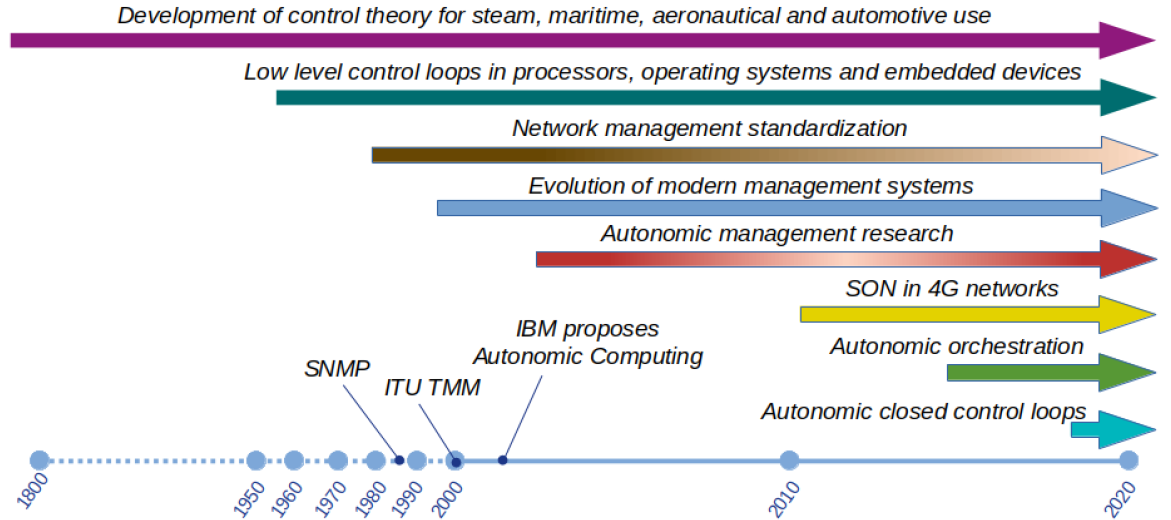
\includegraphics[width=1.0\linewidth]{24-his.png}
    \caption{Zestawienie lini czasu rozwoju systemów zarządzania siecią oraz pętli sterowania. Źródło: \cite{fallon2019}.}\label{fig:24-his}
\end{figure}

\cite{fallon2019} wskazuje wyzwania jakim należy się przeciwstawić, aby umożliwić autonomiczność poprzez pętle sterowania w sieciach. Są to następujące kroki:
\begin{itemize}\hypertarget{list:1}{}
    \item Potrzebny jest model opisujący pętle sterowania w standardowy sposób. Pozwoli to uchronić się przed pragramtycznością i niesystematycznością.
    \item Potrzebny jest framework do wdrażania pętli sterowania umożliwiający ich zarządzanie oraz działanie (ang. \textit{runtime}) w jednym miejscu.
    \item Potrzebne są (najlepiej) graficzne narzędzia do projektowania i symulacji pętli sterowania, tak aby ich wdrażanie nie wymagało specjalistycznych umiejętności technicznych.
\end{itemize}

\subsubsection{ONAP/CLAMP}

Kolejnym zagadnieniem omawianym w \cite{fallon2019} jest system zarządzania ONAP\footnote{\url{https://www.onap.org}} (Open Network Automation Platform) \cite{onap2018}. ONAP to otwartoźródłowa platforma do orkiestracji, zarządzania i automatyzacji usług sieciowych, rozwijana przez fundację Linux Foundation. ONAP składa się z wielu modułów, które umożliwiają pełne zarządzanie cyklem życia usług sieciowych, od ich projektowania, poprzez wdrażanie, aż po operacje eksploatacyjne. Jego kluczowe elementy to:
\begin{itemize}
    \item \textbf{Master Service Orchestrator (MSO)} – centralny moduł odpowiedzialny za orkiestrację usług sieciowych,
    \item \textbf{SDN Controllers (APPC, SDNC, VFC)} –  kontrolery odpowiedzialne za zarządzanie warstwami sieciowymi,
    \item \textbf{A\&AI (Active and Available Inventory)} – moduł odpowiedzialny za inwentaryzację zasobów sieciowych,
    \item \textbf{DCAE (Data Collection, Analytics and Events)} – moduł odpowiedzialny za zbieranie danych, analizę oraz obsługę pętli sterowania,
    \item \textbf{CDS (Controller Design Studio)} – oduł umożliwiający modelowanie inteligentnych konfiguracji sieciowych,
    \item \textbf{CLAMP (Control Loop Automation Management Platform)} – moduł zarządzający zamkniętymi pętlami sterowania.
\end{itemize}

Komponentem odpowiedzialnym za pętle sterowania w ONAP, a jednocześnie kandydatem do rozwiązania wyzwań przedstawionych powyżej, jest CLAMP\footnote{\url{https://docs.onap.org/projects/onap-policy-parent/en/istanbul/clamp/clamp/clamp-architecture.html}}. Jednak posiada on pewne ograniczenia:
\begin{itemize}
    \item Wymaga stosowania architektury pętli zgodnej z modelem MAPE-K, co ogranicza możliwość implementacji niestandardowych pętli sterowania.
    \item Wymaga ścisłej integracji z innymi modułami ONAP, takimi jak DCAE, CDS czy silniki polityk, co ogranicza możliwość implementacji pętli niezależnych od ekosystemu ONAP.
    \item Jest zoptymalizowany pod kątem prostych pętli sterowania. Brak natywnego wsparcia dla bardziej złożonych architektur jak pętle hierarchiczne, rozproszone lub współzależne.
    \item Brak natywnego wsparcia dla sztucznej inteligencji i uczenia maszynowego (AI/ML) w komponentach.
    \item Ścisłe powiązanie z wybranymi silnikami polityk, takimi jak XACML \footnote{\url{https://docs.onap.org/projects/onap-policy-parent/en/istanbul/xacml/xacml.html}}, Drools\footnote{\url{https://docs.onap.org/projects/onap-policy-parent/en/istanbul/drools/drools.html}} czy APEX \footnote{\url{https://docs.onap.org/projects/onap-policy-parent/en/istanbul/apex/apex.html}} 
    \item Silna specjalizacja w orkiestracji sieci SDN i NFV utrudnia rozwój pętli niezwiązanych z tym zagadnieniem.
\end{itemize}

\subsubsection{Architektura referencyjna ETSI ZSM}\hypertarget{sec:zsm}{}
Nadrzędnym celem projektowym ZSM jest umożliwienie zarządzania siecią i usługami w sposób niewymagający ingerencji człowieka (zero touch) w środowisku wielu dostawców (ang. \textit{multi-vendor environment}) \cite{etsizsm2018}. Architektura przyjmuje pewien zestaw pryncypiów (zasad):
\begin{enumerate}\hypertarget{list:2}{}
    \item Modularność  
    \item Rozszerzalność  
    \item Skalowalność  
    \item Sterowane modelem, otwarte interfejsy  
    \item \textbf{Automatyzacja zarządzania w pętli zamkniętej}  
    \item Obsługa funkcji zarządzania bezstanowego  
    \item Odporność  
    \item Rozdzielenie obszarów zarządzania  
    \item Kompozycyjność usług  
    \item Interfejsy oparte na intencjach  
    \item Abstrakcja funkcjonalna  
    \item Prostota  
    \item Zaprojektowane do automatyzacji  
\end{enumerate}

Framework ZSM wpisuje się w trend branżowy polegający na odejściu od monolitycznych, silnie powiązanych systemów na rzecz bardziej elastycznych zestawów usług zarządzania (ang. \textit{management services}). Referencyjna architektura ZSM definiuje zestaw elementów składowych (ang. \textit{building blocks}), które wspólnie umożliwiają konstruowanie bardziej złożonych usług i funkcji zarządzania. Konstrukcja ta odbywa się zgodnie ze wzorcami kompozycji i współdziałania (ang. \textit{composition and interoperation patterns}). 

Framework ZSM składa się logicznie z rozproszonych serwisów zarządzania (ang. \textit{management services}) i serwisów danych (ang. \textit{data services}), które zorganizowane są w domeny zarządzania (ang. \textit{management domains}) oraz zintegrowane poprzez powłokę integracyjną (ang. \textit{integration fabric}). Powłoka integracyjna umożliwia również komunikację serwisów zarządzania z systemami zewnętrznymi.

Architektura referencyjna zapewnia środki do budowania i komponowania luźno powiązanych funkcji zarządzania (ang. \textit{management functions}), które oferują serwisy zarządzania i wspólnie zapewniają kompleksowe zarządzanie danej domeny w sposób "zero-touch". Aby udostępniać swoje usługi, funkcje zarządzania umożliwiają ich wywoływanie oraz komunikację za pomocą punktów końcowych (ang. \textit{endpoints}).

\begin{figure}[!htbp]
    \centering 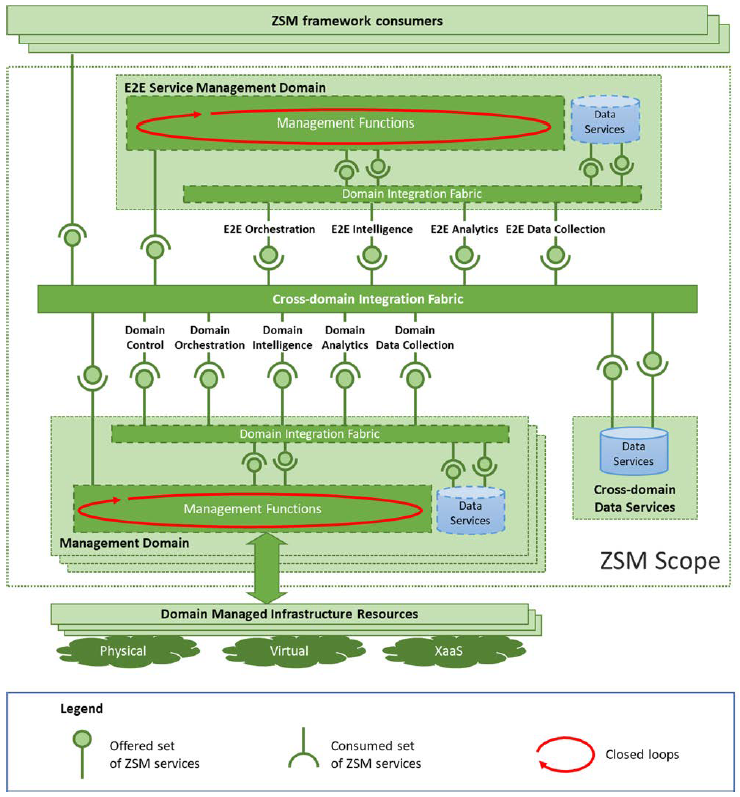
\includegraphics[width=1.0\linewidth]{24-zsm-arch.png}
    \caption{Architektura referencyjna ZSM. Źródło: \cite{etsizsm2018}.}\label{fig:24-zsm-arch}
\end{figure}

Na rysunku \ref{fig:24-zsm-arch} przedstawiono architekturę referencyjną. Poniżej znajduje się krótkie omówienie jej elementów:
\begin{itemize}
    \item Serwis zarządzania (ang. Management Service) - niewidoczna na rysunku, najmniejsza jednostka usługowa architektury, odpowiedzialna za niepodzielny aspekt składowy zarządzania.
    \item Serwis danych (ang. Data Service) - jednostka odpowiedzialna za gromadzenie danych, informacji oraz wiedzy.
    \item Funkcja zarządzania (ang. Management Function) - połączenie wielu serwisów zarządzania, odpowiedzialna za dany aspekt składowy zamkniętej pętli zarządzania.
    \item Domena Zarządzania (ang. Management Domain) - odpowiedzialna za konkretną funkcjonalność zarządzania (np. analityka, orkiestracja, bezpieczeństwo).
    \item Domena Zarządzania end-to-end (ang. E2E Management Domain) - odpowiedzialna za zarządzanie usługami wymagającymi wielu funkcjonalności.
    \item Powłoka Integracyjna (ang. Integration Fabric) - odpowiedzialna za komunikację pomiędzy między wszystkimi komponentami.
\end{itemize}

Pętle zarządzania komponowane są z funkcji zarządzania w sposób pokazany na rysunku \ref{fig:24-zsm-loop}.Za model odniesienia przyjęto strukturę pętli OODA \cite{boyd1995}, rozszerzoną o komponent wiedzy znany z MAPE-K \cite{kephart2003}.

\begin{figure}[!htbp]
    \centering 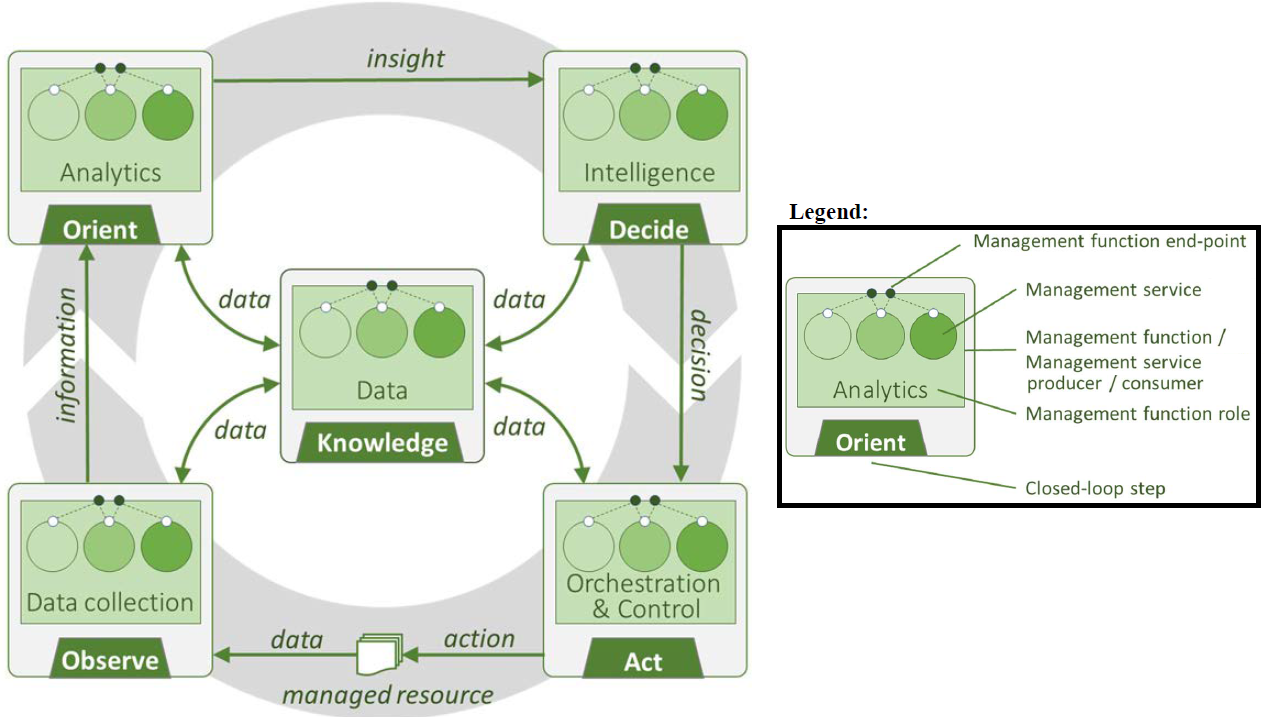
\includegraphics[width=1.0\linewidth]{24-zsm-loop.png}
    \caption{Mapowanie pomiędzy elementami składowymi architektury ZSM a zamkniętą pętlą sterowania. Źródło: Opracowanie własne na postawie \cite{etsizsm2019}.}\label{fig:24-zsm-loop}
\end{figure}


Architektura ZSM określa także cykl życia zamkniętych pętli sterowania oraz mechanizmy ich koordynacji. „Cykl życia pętli podzielony jest na dwie fazy: Design-Time oraz Run-Time. Ich poszczególne etapy przedstawiono na rysunku \ref{fig:24-zsm-lifecycle}. W zakresie koordynacji między pętlami wyróżnia się dwa przypadki: pętle hierarchiczne oraz pętle peer-to-peer. Pętle mogą komunikować się zarówno w obrębie jednej domeny zarządzania, jak i między domenami.

\begin{figure}[!htbp]
    \centering 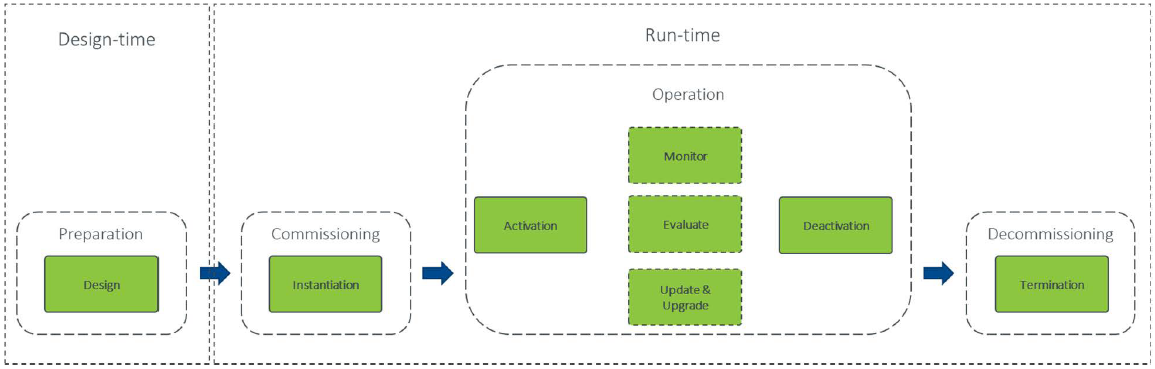
\includegraphics[width=1.0\linewidth]{24-zsm-lifecycle.png}
    \caption{Fazy cyklu życia oraz aktywności zamkniętej pętli sterowania. Źródło: \cite{etsizsm2019}.}\label{fig:24-zsm-lifecycle}
\end{figure}




\subsubsection{Architektura referencyjna CLADRA (TM Forum)}\hypertarget{sec:cladra}{}

TM Forum definiuje architekturę referencyjną, która, wykorzystując zamknięte pętle sterowania, umożliwia szybkie wykrywanie oraz rozwiązywanie problemów w sieciach. Podobnie jak architektura ETSI ZSM, bazuje na Open Digital Architecture (ODA) \cite{tmforum2018}. CLADRA jednakże to ogólna koncepcja architektoniczna i zestaw dobrych praktyk, a nie formalna specyfikacja techniczna jak ETSI ZSM.

W \cite{tmforum2021} przedstawiono architekturę logiczną (Rysunek \ref{fig:24-tmforum-arch}).

\begin{figure}[!htbp]
    \centering 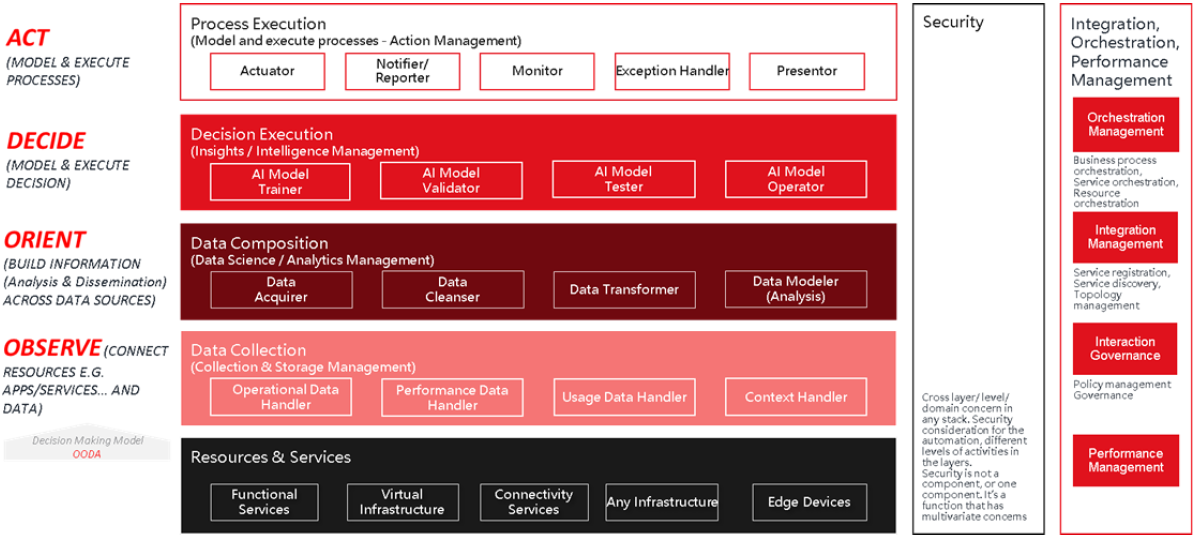
\includegraphics[width=1.0\linewidth]{24-tmforum-arch.png}
    \caption{Architektura logiczna CLADRA. Źródło: \cite{tmforum2021}.}\label{fig:24-tmforum-arch}
\end{figure}

Jej podstawą jest pętla OODA. Faza „Observe” odpowiada za zbieranie danych z sieci, które następnie, w wyniku analizy, są przekształcane w informację w fazie „Orient”. W fazie „Decide” podejmowane i modelowane są decyzje, które przekładają się na konkretne workflow do realizacji. Faza "Act" orkiestruje wykonaniem workflow na zarządzanych zasobach. Istotnym aspektem jest to, że (workflow) dla akcji rekoncyliacyjnych jest wyznaczany dynamicznie podczas iteracji pętli, w przeciwieństwie do przepływu pracy zdefiniowanego przed uruchomieniem danej iteracji. 

Architektura ta operuje na innym poziomie abstrakcji niż ZSM. Konkretne jej implementacje przedstawione w \cite{tmforum2022} różnią się bardzo od siebie i tak jak wskazano w \cite{fallon2019} są bardzo sztywne i skierowane na dany use-case. Podobnie jak w architekturze ETSI ZSM, przewiduje się uruchamianie wielu instancji pętli jednocześnie na jednym logicznie oddzielnym komponencie. Celem tych pętli jest autonomiczne zarządzanie, realizowane za pomocą komunikacji z zewnętrznymi względem tego komponentu zasobami.

\cite{tmforum2022ai} prezentuje koncepcję Menedżera Zamkniętych Pętli (ang. \textit{Closed Loop Manager}), czyli logicznego komponentu architektury odpowiedzialnego za zarządzanie pętlami sterowania. Podobna kwestia poruszana jest również przez \cite{ngmn2022}. Taki menadżer w kontekście pętli sterowania jest odpowiedzialny za:
\begin{itemize}
    \item Zarządzanie ich cyklem życia 
    \item Konfiguracje ich celów zarządzania
    \item Monitorowanie ich stanu
\end{itemize}

Pełna tabela funkcjonalności proponowanych dla Menadżera Zamkniętych Pętli przez TM Forum znajduje się w \hyperlink{appendix:11}{Załączniku 11}.

\subsubsection{Achitektura referencyjna ETSI ENI}

ENI rozwija specyfikacje dotyczące Kognitywnego Systemu Zarządzania, który będzie samodzielnie regulował działanie sieci poprzez wykorzystanie technik sztucznej inteligencji, takich jak \hyperlink{def:uczenie-maszynowe}{uczenie maszynowe (ang. \textit{machine learning})} oraz \hyperlink{def:wnioskowanie}{wnioskowanie (ang. \textit{reasoning})}. 

Z poprzedniego rozdziału wiemy, że aby \hyperlink{def:wnioskowanie}{\textit{wnioskować}} potrzebna jest \hyperlink{def:wiedza}{\textit{wiedza}}. Skąd taki system pozyskiwałby wiedzę? Otóż, dzieje się to poprzez proces \hyperlink{def:uczenie-maszynowe}{\textit{Uczenia Maszynowego}}. Pierwsza faza, czyli tzw. "trening", odbywa się przed wdrożeniem systemu. System może także uczyć się na podstawie doświadczenia (ang. \textit{experience}), gdy już jest w pełni operacyjny. Dlatego mówimy o empirycznej inteligencji sieciowej (ang. \textit{experiential networked intelligence}). 

Architekturę \cite{etsieni2023} ENI obrazuje Rysunek \ref{fig:24-eni-arch}. Fioletowe komponenty są zewnętrzne dla systemu ENI: górny stanowi jednostki zlecające mu zarządzanie, zaś dolny zarządzany obiekt (w tym przypadku zarządzana infrastruktura). Pomiędzy nimi występują pętle zarządzania end-to-end, co jest koncepcją zbliżoną do ETSI ZSM. Oba komponenty zewnętrzne, ponieważ sieci telekomunikacyjne funkcjonują w środowisku wielu dostawców (ang. \textit{multi-vendor environment}), muszą przejść proces normalizacji formatu danych i interfejsów do jednolitego formatu rozumianego przez ENI System (tzw. ENI Format). Odpowiedzialne za to są dwa czerwone komponenty. Kluczowym elementem architektury jest zielony komponent. To w tym komponencie realizowane są operacje zarządzania oparte na sztucznej inteligencji. Cały cykl zamyka pętla sterowania. 

Podczas gdy ZSM definiuje framework do orkiestracji i egzekwowania działań w sieci, ENI może pełnić funkcję warstwy kognitywnej dla ZSM. ZSM realizuje zamknięte pętle sterowania, reagując na konkretne zdarzenia w czasie rzeczywistym. ENI analizuje długoterminowe trendy i dynamicznie dostosowuje polityki zarządzania, na przykład w celu zapobiegania anomaliom sieciowym. \hyperlink{def:kognitywnosc}{\textit{Kognitywność}} ENI również opiera się na zamkniętych pętlach sterowania. Co istotne z punktu widzenia niniejszej pracy, \cite{etsieni2024} dokonuje przeglądu różnych architektur zamkniętych pętli sterowania, które mogą zostać wykorzystane w systemie ENI. Stanowi cenne źródło wiedzy na temat charakterystyk zamkniętych pętli sterowania. Jego analiza znajduje się w \hyperlink{sec:25}{następnym podrozdziale}.



\begin{figure}[!h]
    \centering 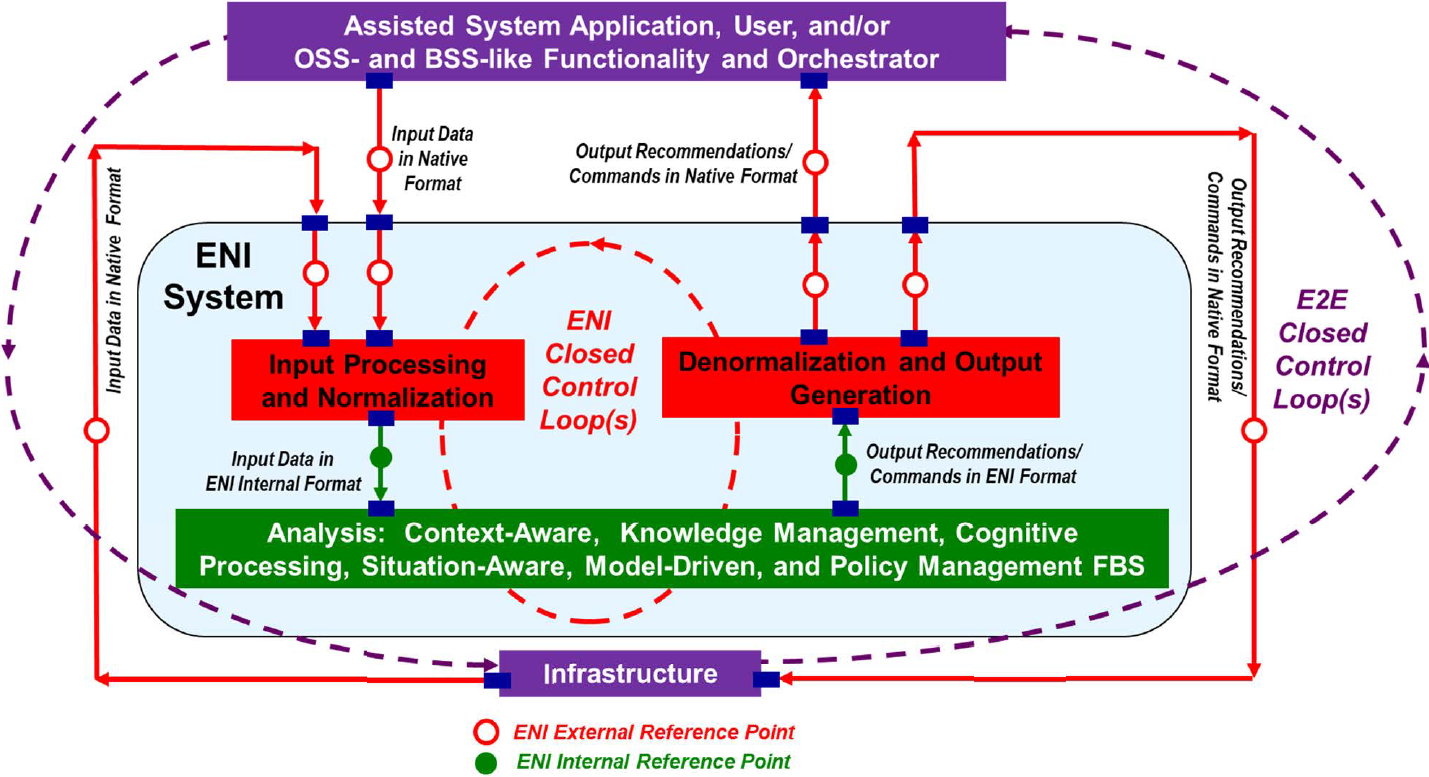
\includegraphics[width=1\linewidth]{24-eni-arch.png}
    \caption{Wysokopoziomowa architektura funkcjonalna ENI. Źródło: \cite{etsieni2023}.}\label{fig:24-eni-arch}
\end{figure}


\subsubsection{Podsumowanie}

Niniejsza praca identyfikuje lukę, którą zamierza wypełnić poprzez opracowanie platformy umożliwiającej modelowanie, uruchamianie oraz zarządzanie zamkniętymi pętlami sterowania. Luka ta umotywowana jest \hyperlink{list:1}{wyzwaniami zdefiniowanymi przez \cite{fallon2019}}, brakami w ONAP/CLAMP oraz zidentyfikowania takiej potrzeby w architekturach referencyjnych ETSI oraz CLADRA.

Proponowana w niniejszej pracy platforma, inspirowana architekturą z \cite{kephart2003}, opiera się na scentralizowaniu autonomicznych menedżerów na wspólnej platformie (Rysunek \ref{fig:24-lupus}).

\begin{figure}[!htbp]
    \centering 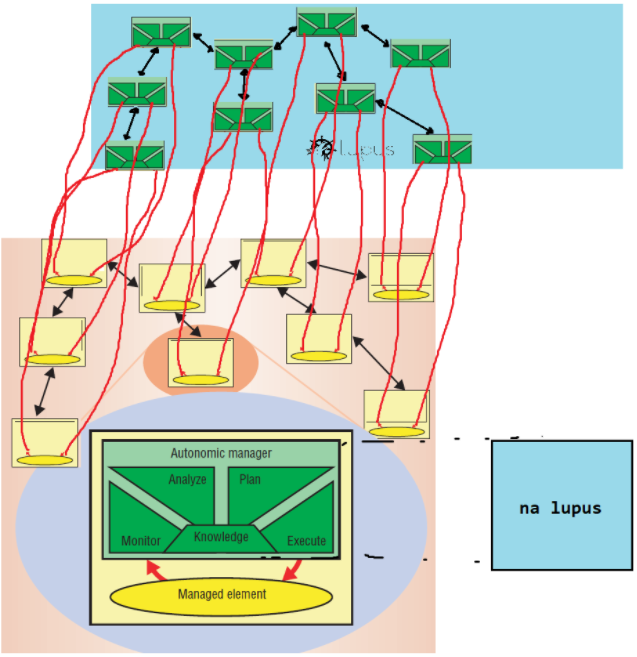
\includegraphics[width=1.0\linewidth]{24-lupus.png}
    \caption{Koncepcja wyniesienia autonomicznych menadżerów na wspólną platformę. Źródło: Opracowanie własne na podstawie: \cite{kephart2003}.}\label{fig:24-lupus}
\end{figure}